\documentclass[fleqn,10pt]{wlscirep}
\usepackage[utf8]{inputenc}
\usepackage[T1]{fontenc}
\usepackage{lineno}
\usepackage{float}
\linenumbers

\providecommand{\tightlist}{%
  \setlength{\itemsep}{0pt}\setlength{\parskip}{0pt}}


\newlength{\cslhangindent}
\setlength{\cslhangindent}{1.5em}
\newenvironment{CSLReferences}%
{\setlength{\parindent}{0pt}%
\everypar{\setlength{\hangindent}{\cslhangindent}}\ignorespaces}%
{\par}

\title{Multiorder Hydrologic Position in Europe as a Set of Metrics in Support of Groundwater Mapping at Regional and National Scales}

\author[*, 1]{Maximilian Nölscher}
\author[2]{Michael Mutz}
\author[1]{Stefan Broda}
\affil[1]{Federal Institute for Geosciences and Natural Resources (BGR), Sub-Department: Basic information Groundwater and Soil (B2.2), Berlin, 13593, Germany}
\affil[2]{independet researcher}
\affil[*]{corresponding author: Maximilian Nölscher (max-n@posteo.de)}


\begin{abstract}
This dataset (EU-MOHP v013.0.1) provides information on the multiorder hydrologic position of a geographic point within its respective river network and catchment. More precisely, it comprises the three measures ``lateral position'' as a relative measure of the position between the stream and the catchment boundary/ watershed, ``divide stream distance'' as an absolute distance measure that serves as a proxy for the position within the catchment and ``stream distance'' as an absolute measure of the distance to the nearest stream. These three measures were calculated for several hydrologic (stream) orders and therefore reflecst different spatial scales. Its spatial extent covers major parts of physiographical Europe and all of the 39 countries in European Economic Area (EEA39). Although there might be many potential use cases, this dataset serves predominantly as valuable static geophysical or environmental predictor variable among other input data for mapping or modeling tasks in the context of hydrogeology and hydrology.
\end{abstract}
\begin{document}

\flushbottom
\maketitle
%  Click the title above to edit the author information and abstract

\thispagestyle{empty}

\hypertarget{background-summary}{%
\section{Background \& Summary}\label{background-summary}}

In recent years, data science tools such as machine learning are increasingly applied to and specifically developed for hydro(geo)logical challenges and research questions (!!source: Zounemat 2020). In the field of hydrogeology, machine learning has been used successfully for groundwater level prediction and a variety of mapping tasks (!!source: wunsch 2021; knoll, desimone). Since machine learning models -- except for hydrid- or physics-guided models -- are purely based on data with no built-in knowledge of physical processes, it is important to provide as many features (synonyms: predictor variables, explanatory variables) as possible that have an impact on the target variable to potentially enable the machine learning algorithm to reproduce the result of the underlying process. For surface and near-surface processes, this criterion may be more or less satisfiable through the availability of remote sensing data, whereas for modeling subsurface processes such as in hydrogeology, this poses a serious challenge.

The key motivation of this dataset is to provide a set of features that introduce hydrological context to machine learning models regarding the horizontal position of a point within its catchment. Therefore, it functions as a proxy for multiple geophysical characteristics of a hydrologic system. It complements commonly available data sets and tackles the above mentioned challenge.
This dataset is strongly inspired by {[}!!source: Beelitz et. al.{]} and adapts their ideas and methods to the ``EU-Hydro - River Network Database'' but -- in contrast -- with purely free open source software and a strong focus on reproducibility. {[}!!source: Beelitz et. al.{]} provides a comprehensive explanation of the motivation as well as a detailed discussion for further reading.

In their study, Belitz et al. (2019) also provide the results from case studies to proof that the multiorder hydrologic position is a valuable feature when mapping divers geophysical targets using machine learning. Its benefit to the performance of machine learning models has also been acknowledged by several other studies {[}!!source: Using Boosted Regression Tree Models to Predict Salinity in Mississippi Embayment Aquifers, Central United States; Machine Learning Predictions of pH in the Glacial Aquifer System, Northern USA; Machine-learning models to map pH and redox conditions in groundwater in a layered aquifer system, Northern Atlantic Coastal Plain, eastern USA; The relation of geogenic contaminants to groundwater age, aquifer hydrologic position, water type, and redox conditions in Atlantic and Gulf Coastal Plain aquifers, eastern and south-central USA{]}.

Being a static geophysical catchment attribute, the EU-MOHP data set can be used as features in any machine learning task in the domain of hydrology and hydrogeology. Because of the calculation based on the different streamorders, this data set can be applied for multiple spatial scales and depths -- from local via regional to continental scales. Examples of use cases might be the mapping of hydrogeochemical parameters or hydraulic variables like depth to groundwater, the prediction of groundwater levels or catchment classification tasks using unsupervised machine learning methods.

The EU-MOHP v013.0.1 data set comprises the 3 measures

\begin{itemize}
\tightlist
\item
  lateral position (lp)
\item
  divide stream distance (dsd) and
\item
  stream distance (sd)
\end{itemize}

for each of the 6 streamorders which leads to \(n_{measures}n_{streamorders} = 18\) different metrics to be used as features. Spatially, the data set covers major parts of physiographical Europe and all of the 39 countries in European Economic Area (EEA39). More precisely, it covers the 2 largest coherent land masses of the EEA39 (see fig.~\ref{fig:studyareafigure}).

The generation of this data set is based on two basic data products which are the ``EU-Hydro -- River Network Database'' and ``EU-Hydro -- Coastline'' with the advantage that the dependencies are low from a data point of view. Therefore, it is possible to transfer the methodology to other regions with only little effort. For the calculation of the MOHP metrics in general, the following 4 essential data layers are required:

\begin{enumerate}
\def\labelenumi{\arabic{enumi}.}
\tightlist
\item
  \textbf{river network} as vector layer with linestring geometries
\item
  \textbf{surface water bodies} such as lakes as vector layer with polygon geometries
\item
  respective \textbf{river basins} as vector layer with polygon geometries
\item
  \textbf{coastline} as vector layer with linestring geometries
\end{enumerate}

These data layers are the basis for all further calculations of this data set. In this case, they were all obtained from the mentioned data sources provided by Copernicus Land Monitoring Service. The data set was manually downloaded from the website of Copernicus - Land Monitoring Service ({``{EU}-{Hydro} - {Coastline}''} 2021) and subsequently processed in the R programming language (see fig.~\ref{fig:workflowfigure}; R Core Team 2020). Due to the memory size of this data set as well as for the sake of computational speed, a PostgreQL database with PostGIS extension was used for some processing steps of vector data and GRASS GIS database was used for all final calculations of the MOHP metrics (see fig.~\ref{fig:workflowfigure}D and E). For reproducability and control reasons, all processing steps including the databases were tracked and executed through a data processing pipeline using the targets package in R (see fig \ref{fig:workflowfigure}; Landau 2021). More details can be found in \protect\hyperlink{methods}{Methods} or in the code itself (see \protect\hyperlink{code-availability}{Code availability}).

\hypertarget{methods}{%
\section*{Methods}\label{methods}}
\addcontentsline{toc}{section}{Methods}

The methods will be described by following the chronological order of the processing steps in the targets pipeline as it can be found in the code. This order is mainly guided by the dependencies of the processing steps. To better refer to the code, each processing step is provided with a paragraph naming its respective target names in the targets pipeline. The single processing steps are thematically summarised. The targets pipeline is split across multiple files in the \texttt{targets} directory (see \ref{fig:projectdirtree}, line 28) and merged in \texttt{\_targets} (see \ref{fig:projectdirtree}, line 39). For more details, see these files. The targets marked \texttt{(helper\ target)} are not described here because they are not relevant to the methods and exist only for technical reasons.

\hypertarget{overview}{%
\subsection{Overview}\label{overview}}

The methods of this study conceptually follows the methods described in Belitz et al. (2019) which we highly recommend for further reading. The

@ref(fig:projectdirtree

\hypertarget{data-acquisition}{%
\subsection{Data Acquisition}\label{data-acquisition}}

The required river network data ``EU-Hydro -- River Network Database'' as well as the coastline were manually downloaded from the Copernicus - Land Monitoring Service website ({``{EU}-{Hydro} - {Coastline}''} 2021, 2021). This step relates to fig.~\ref{fig:workflowfigure}A. The unzipped files have a size of approximately 14 GB.

\hypertarget{processing-steps}{%
\subsection{Processing Steps}\label{processing-steps}}

All following steps relate to fig.~\ref{fig:workflowfigure}C, D, and E.

\hypertarget{data-import}{%
\subsubsection{Data import}\label{data-import}}

In this study, we used the coordinate reference system (CRS) ETRS89-extended / LAEA Europe with the EPSG code 3035. Therefore, all data was reprojected to this CRS after importing in case it differed.

\hypertarget{river-networks}{%
\paragraph{River networks}\label{river-networks}}

\hypertarget{detailed-workflow}{%
\subsection*{Detailed Workflow}\label{detailed-workflow}}
\addcontentsline{toc}{subsection}{Detailed Workflow}

In the following, the description of the methods is oriented towards the structure of the targets pipeline to easily relate the methods description here to the source code in the repository. All steps required to understand the workflow will be described, for further details we refer to the source code.

\hypertarget{step-1-data-acquisition}{%
\subsubsection*{Step 1: Data Acquisition}\label{step-1-data-acquisition}}
\addcontentsline{toc}{subsubsection}{Step 1: Data Acquisition}

The ``EU-Hydro - River Network Database'' was manually downloaded from \url{https://land.copernicus.eu} (for detailed link see references) as version v013. All downloaded and unzipped files have approximately 14 GB. The !!river is the only underlying data for the generation of the EU-MOHP dataset.

\hypertarget{hardware}{%
\subsection*{Hardware}\label{hardware}}
\addcontentsline{toc}{subsection}{Hardware}

The pipeline to generate the data set was executed on a DELL PowerEdge C4140 Server with an Intel Xeon Gold 6240R CPU and 384 GB installed RAM. The installed operation system is Microsoft Windows Server 2019 Standard, version 10.0.17763 Build 17763.

{[}what is different to the Beelitz Paper and why{]}
NHDPlusV2 data
No pathleveId column
Criterion to exclusively use free open source software

\hypertarget{data-records}{%
\section*{Data Records}\label{data-records}}
\addcontentsline{toc}{section}{Data Records}

Text.

\hypertarget{technical-validation}{%
\section*{Technical Validation}\label{technical-validation}}
\addcontentsline{toc}{section}{Technical Validation}

Text.

\hypertarget{usage-notes}{%
\section*{Usage Notes}\label{usage-notes}}
\addcontentsline{toc}{section}{Usage Notes}

Text.

\hypertarget{code-availability}{%
\section*{Code availability}\label{code-availability}}
\addcontentsline{toc}{section}{Code availability}

All processing and analysis was conducted with free open source software. All processing steps except for the download of the ``EU-Hydro - River Network Database'' (for practical reasons also referred to as river database) that was done manually are controlled and executed from within a targets pipeline in the programming language R {[}see fig.~!!source{]}. Targets is an R package that provides a toolkit for reproducible workflows {[}!!source{]}. Spatial vector data such as the EU-Rivers are processed partly in R and a PostgreSQL (version 13) database with PostGIS (version 3.1.0) extension database for speed and memory reasons. For the same reason, all major raster calculations were conducted in a GRASS GIS (version 7.8.5-2) database. The database connections and all calculations in the databases are also controlled by this pipeline. For reaching a maximum of reproducibility, a docker container is provided to rerun all calculations easily. The R package renv is used for keeping track of the required R package versions and fits well to the combination with targets and docker to endure reproducibility.

\hypertarget{acknowledgements}{%
\section*{Acknowledgements}\label{acknowledgements}}
\addcontentsline{toc}{section}{Acknowledgements}

Text.

\hypertarget{author-contributions-statement}{%
\section*{Author contributions statement}\label{author-contributions-statement}}
\addcontentsline{toc}{section}{Author contributions statement}

Text.

\hypertarget{competing-interests}{%
\section*{Competing interests}\label{competing-interests}}
\addcontentsline{toc}{section}{Competing interests}

Text.

\hypertarget{figures-tables}{%
\section*{Figures \& Tables}\label{figures-tables}}
\addcontentsline{toc}{section}{Figures \& Tables}

\begin{figure}[H]

{\centering 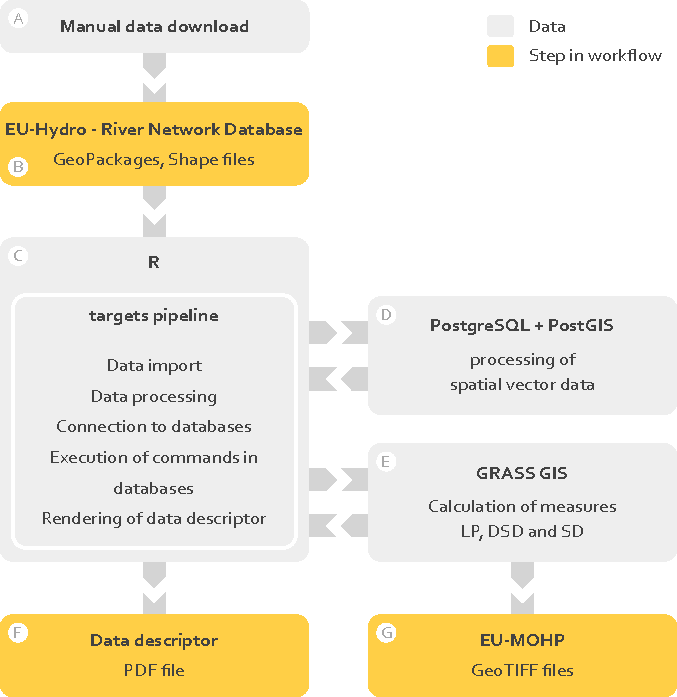
\includegraphics[width=0.7\linewidth]{diagramms/workflow_figure} 

}

\caption{Workflow of the data processing in different software.}\label{fig:workflowfigure}
\end{figure}

\begin{figure}[H]

{\centering \includegraphics[width=0.8\linewidth]{main_files/figure-latex/studyareafigure-1} 

}

\caption{Spatial coverage of this data set. The legend labels show the names according to the file name. If you want to more precisely check wether your study area or area of interest is covered by this dataset, please visit !!link to github readme.}\label{fig:studyareafigure}
\end{figure}

\begin{figure}[H]

{\centering 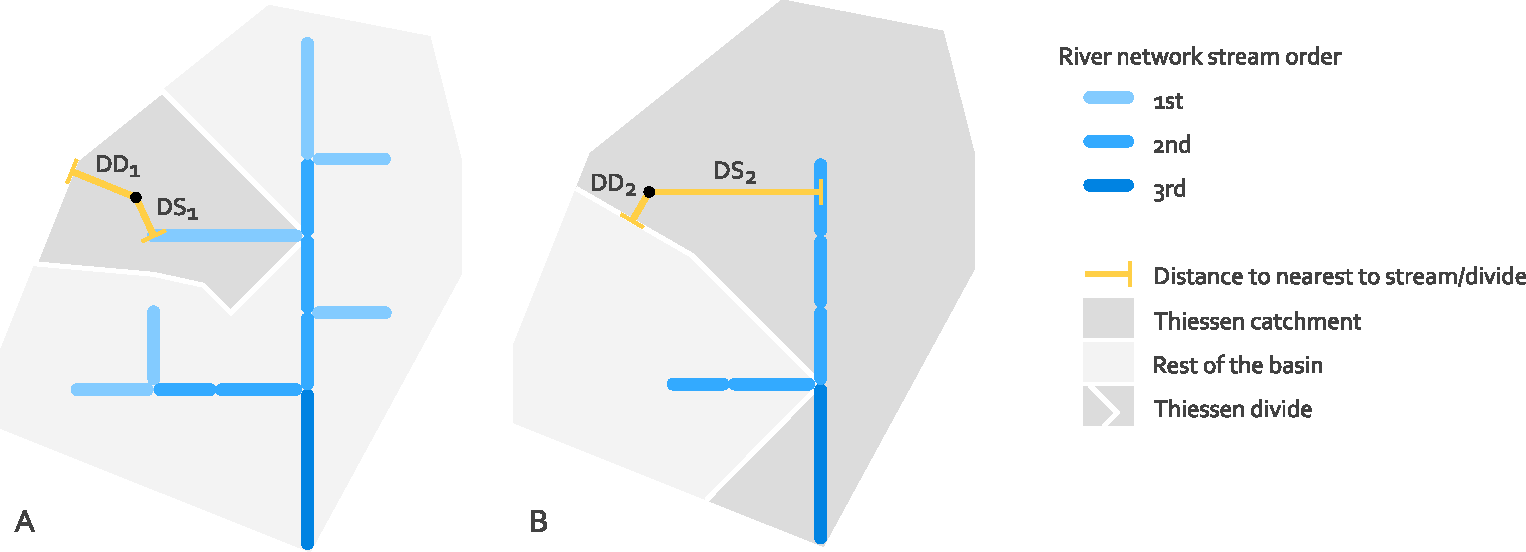
\includegraphics[width=0.8\linewidth]{diagramms/mohp_scheme} 

}

\caption{Schematic representation of MOHP measures using two examples for the stream orders one (A) and two (B)}\label{fig:Schematicmohp}
\end{figure}

\hypertarget{refs}{}
\begin{CSLReferences}{1}{0}
\leavevmode\hypertarget{ref-belitz_multiorder_2019}{}%
Belitz, Kenneth, Richard B. Moore, Terri L. Arnold, Jennifer B. Sharpe, and J. J. Starn. 2019. {``Multiorder {Hydrologic} {Position} in the {Conterminous} {United} {States}: {A} {Set} of {Metrics} in {Support} of {Groundwater} {Mapping} at {Regional} and {National} {Scales}.''} \emph{Water Resources Research} 55 (12): 11188--207. \url{https://doi.org/10.1029/2019WR025908}.

\leavevmode\hypertarget{ref-noauthor_eu-hydro_2021}{}%
{``{EU}-{Hydro} - {Coastline}.''} 2021. \emph{EU-Hydro - Coastline â€'' Copernicus Land Monitoring Service}. \url{https://land.copernicus.eu/imagery-in-situ/eu-hydro/eu-hydro-coastline?tab=download}.

\leavevmode\hypertarget{ref-landau_targets_2021}{}%
Landau, William Michael. 2021. {``The Targets {R} Package: A Dynamic {Make}-Like Function-Oriented Pipeline Toolkit for Reproducibility and High-Performance Computing.''} \emph{Journal of Open Source Software} 6 (57): 2959. \url{https://doi.org/10.21105/joss.02959}.

\leavevmode\hypertarget{ref-r_core_team_r_2020}{}%
R Core Team. 2020. \emph{R: {A} {Language} and {Environment} for {Statistical} {Computing}}. Vienna, Austria: R Foundation for Statistical Computing. \url{https://www.R-project.org/}.

\end{CSLReferences}

\nocite{*}
\bibliography{eumohp.bib}

\end{document}
